\chapter{評価}
{
\label{chap:eval}

\section{評価環境}
\label{sec:eval_env}
実装はVivado HLS(2017.3)を用いて実装を行った.対象となるFPGAボードは\ref{chap:ficsw}章の\ref{sec:about_ficsw}節でも言及した
Xilinx社のKintex Ultrascale XCKU095-FFVB2104である.動作周波数は100MHzとした.
実装対象,ベンチマークとして表\ref{table:googlenet}に示されるInception(3a)層を用いた.
Vivado HLS上でのシュミレーションの実行サイクル数から実行時間を計算した。
比較対象となるCPUはIntel Xeon CPU E5-2667 0(@2.90GHz)を用いて,g++4.4.7でのO3最適化とOpenMPを使って
コンパイルしたアプリケーションの実行時間を計測した.

\section{リソース使用量と割合}
\label{sec:resource_util}
表\ref{table:resource_util}に各スレッドモジュールのFPGA合成結果のリソース使用率を示す.
[]内はその割合を\%で示している..

\begin{table}[p]
    \begin{center}
    \caption{各スレッドにおけるFPGAボードのリソース使用量とその割合}
    \label{table:resource_util}
    \begin{tabular}{|c|c|c|c|c|} \hline
    \multicolumn{1}{|c|}{Thread} & \multicolumn{1}{|c|}{BRAM\_18K} & \multicolumn{1}{|c|}{DSP48} & \multicolumn{1}{|c|}{FF} & \multicolumn{1}{|c|}{LUT} \\ \hline \hline
    Thread1       & 10[1] & 10[1] & 10[1] & 10[1] \\ \hline
    Thread2       & 10[1] & 10[1] & 10[1] & 10[1] \\ \hline
    Thread3       & 10[1] & 10[1] & 10[1] & 10[1] \\ \hline
    Thread4       & 10[1] & 10[1] & 10[1] & 10[1] \\ \hline
    \end{tabular}
    \end{center}
\end{table}


\section{実行時間の比較}
\label{sec:resource_util}

比較対象となるCPU,FPGAにそれぞれGoogLeNetの実装を行い,その実行時間を計測した結果を図\ref{fig:exec_graph}に示す.
グラフの縦軸は実行時間を対数で示している.また詳しい数値は表\ref{table:exec_time}に示す.

\begin{figure}[h]
    \centering
    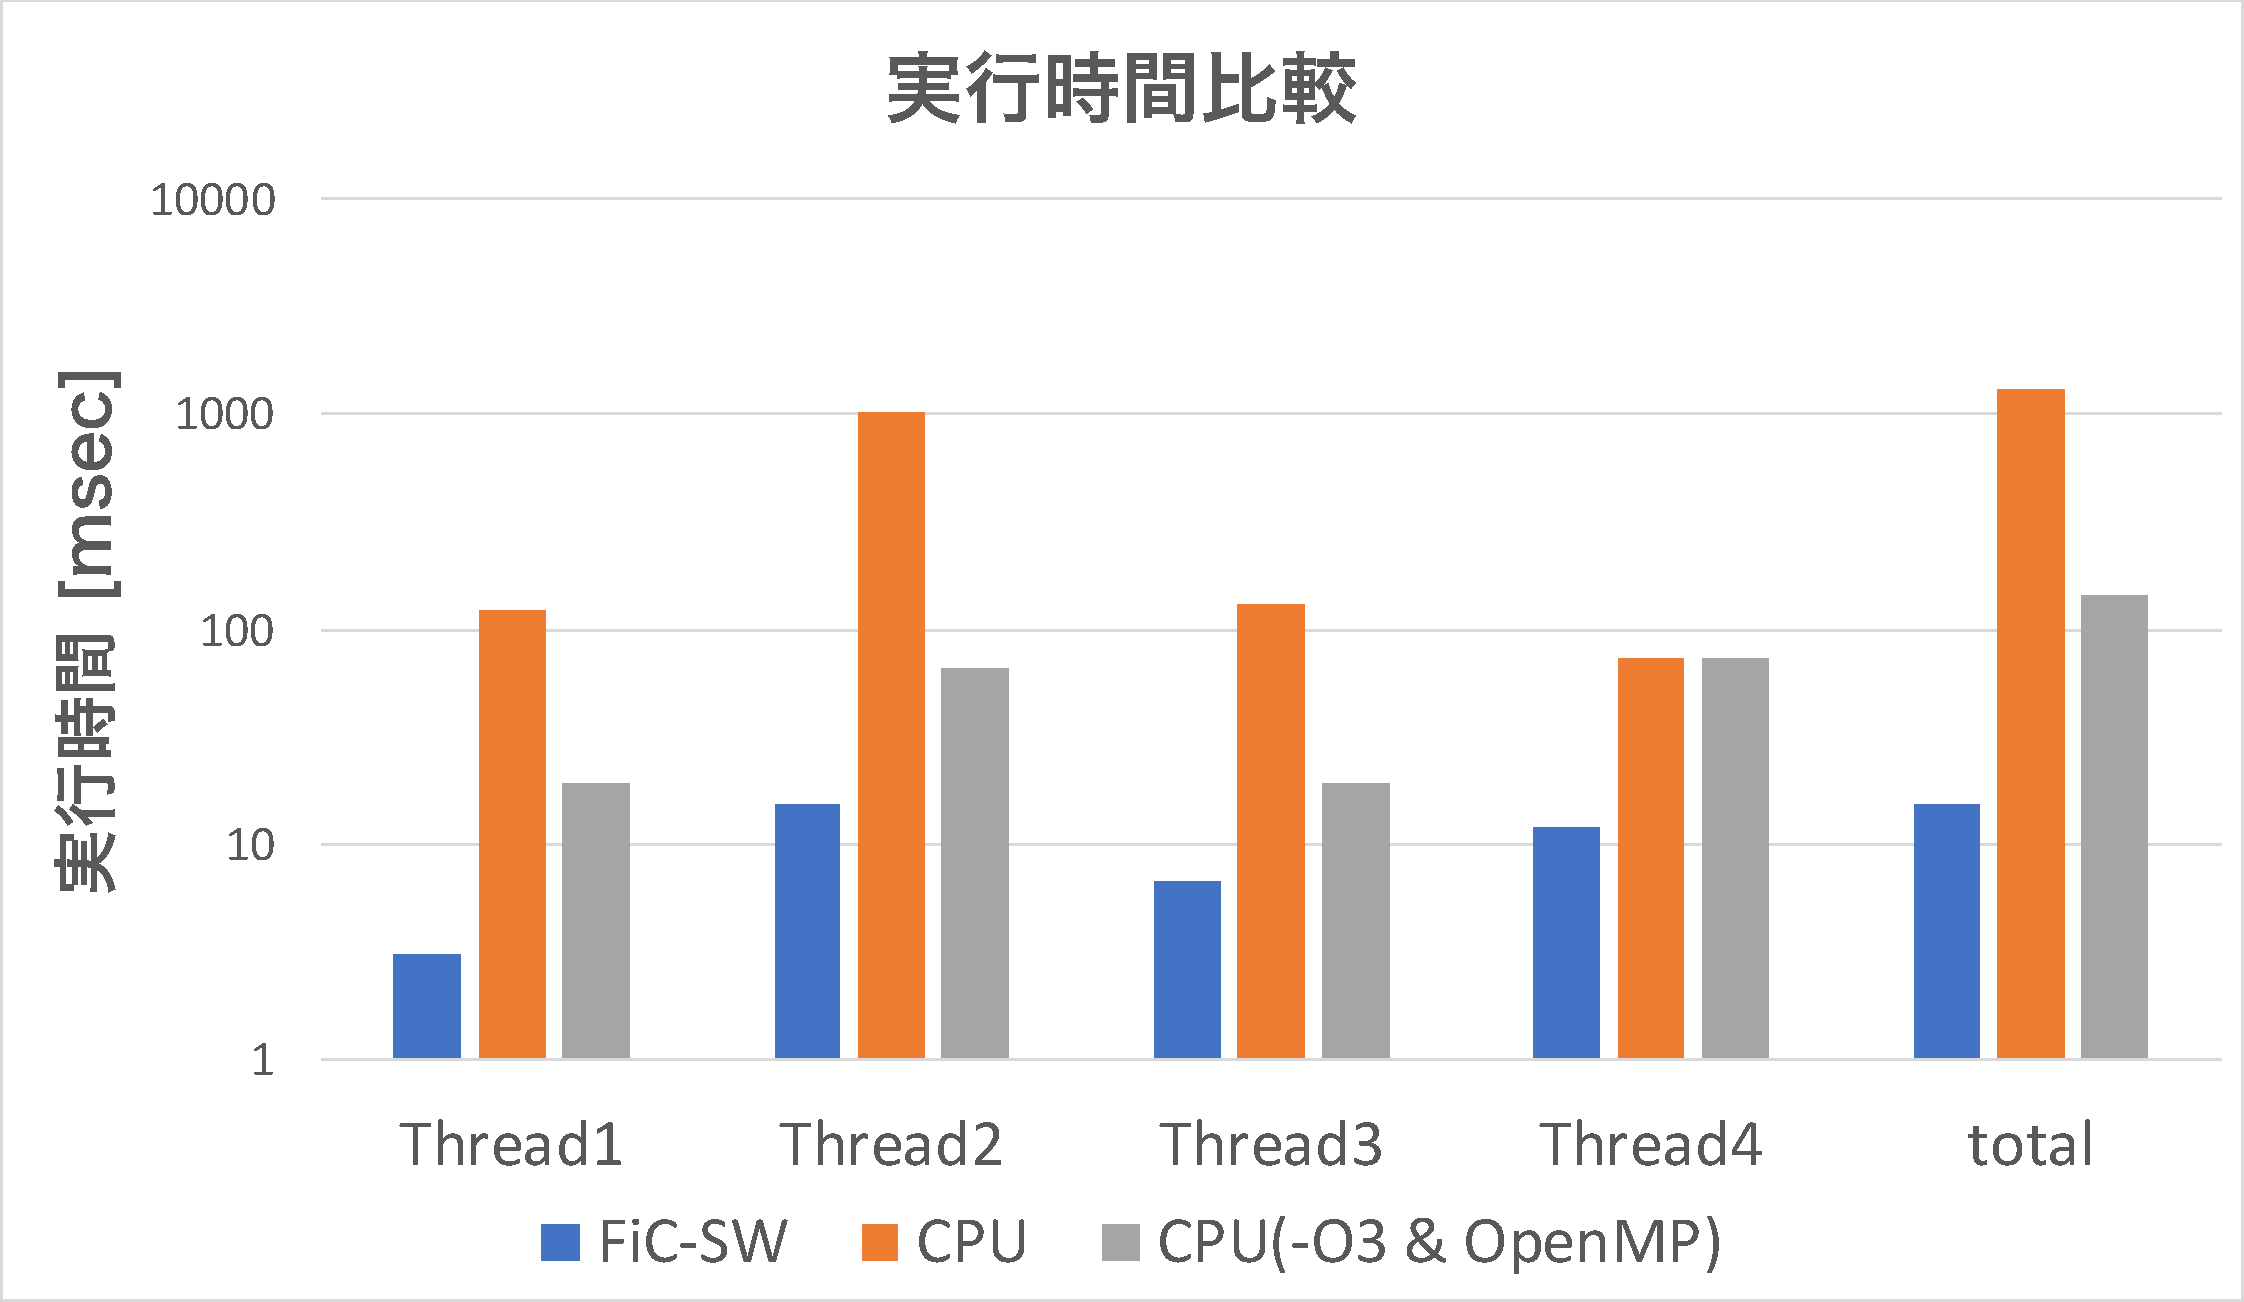
\includegraphics[width=15cm]{./chap7/fig/exec_time.pdf}
    \caption{}
    \label{fig:exec_graph}
\end{figure}

表\ref{table:exec_time}に各スレッドモジュールのFPGA実行時間とCPUでの実行時間を示す.
また全ての演算を行った際の合計の実行時間も示す.

\begin{table}[p]
    \begin{center}
    \caption{各スレッドとInception(3a)層全体の実行時間の比較}
    \label{table:exec_time}
    \begin{tabular}{|c|c|c|c|} \hline
    \multicolumn{1}{|c|}{Thread} & \multicolumn{1}{|c|}{FPGA} & \multicolumn{1}{|c|}{CPU} & \multicolumn{1}{|c|}{CPU -O3 \& OpenMP} \\ \hline \hline
    Thread1       & 10 & 123 & 19 \\ \hline
    Thread2       & 10 & 1022 & 65 \\ \hline
    Thread3       & 10 & 132 & 19 \\ \hline
    Thread4       & 10 & 74 & 73 \\ \hline
    Total         & 10 & 1309 & 142 \\ \hline
    \end{tabular}
    \end{center}
\end{table}

Inception層では前層の出力特徴マップが全て揃うまで演算を行うことができないので
各スレッドはお互いの処理が終了するまでは待機していなければいけない.
そのため,Inception層自体の実行時間は一番処理に時間がかかるスレッドに律速されてしまう.
以上の結果からInception(3a)層において,FiC-SWはOpenMPを利用して最適化を図ったIntel Xeon CPU E5-2667 0(@2.90GHz)に対して,
〇〇倍の高速化を達成した.
}
